\chapter{从滚动标量场产生的暴胀}

\lectureoverview{上一次会议留下的一个问题提供了组织方程，
\(\ddot\phi+3H\dot\phi=-V'(\phi)\)：什么在运动，什么施加力，以及为什么膨胀类似于摩擦？我们首先在固定盒子中推导该方程，然后在膨胀盒子中推导。将其与弗里德曼方程耦合，就得到慢滚机制，其中高而浅的标量势驱动近乎指数的膨胀。暴胀稀释磁单极子并抹平几何；其结束使宇宙重新加热，并开启常规的热大爆炸。那么最后一个问题就不可避免：如果暴胀如此高效地抹平一切，结构又从何而来？一维焦散计算展示了微小的速度变化如何产生片状、纤维状和结状结构，同时将这些变化的量子起源推迟到下一讲。}

\section{什么作用于什么？}

开场问题回顾了方程
\begin{equation}
\ddot\phi+3H\dot\phi
=F(\phi)
=-\frac{dV}{d\phi}
\label{eq:c09-opening}
\end{equation}
并询问什么样的力\(F\)可以作用于一个场。这个问题并非无关紧要。要回答它，我们必须重构场的力学，而在这样做时，我们就开始了暴胀这一主题本身。

标量场为空间和时间的每一点赋予一个数\(\phi(\mathbf x,t)\)。电场和磁场携带能量；标量场也可以携带能量。这里所需的场是假设性的：尚未通过实验识别出任何特定的暴胀子，因此其能量作为场值的函数是未知的。因此，我们用一个未指定的势能密度来表示它
\begin{equation}
V=V(\phi).
\label{eq:c09-potential}
\end{equation}
\(\phi\)的不同值对应于每单位物理体积中储存的不同能量。

没有理由认为\(\phi=0\)具有零能量。场空间的原点是一种约定，尤其对于一个尚未发现的场而言，而移动用于标记场值的坐标并不需要将\(V\)的最小值置于原点。\(V(\phi)\)的图形描述的是相对斜率和高度，而不是场的某个特权起点。

势能是当场瞬时静止时保留下来的部分。如果场随时间变化，它也具有动能。量\(\dot\phi\)不是物体在普通空间中的速度；它是场的值变化的速率，是场空间中的速度。一根弹性弦提供了一个有用的类比。它的位移是一维世界上的一个场，而振动的弦元携带的动能与其时间导数的平方成正比。

该平方的系数可以吸收到场本身的定义中。如果从
\begin{equation}
\frac12 n^2\dot\phi^{\,2},
\end{equation}
开始，那么变量变换
\begin{equation}
\chi=n\phi
\end{equation}
将该术语变为\(\dot\chi^{\,2}/2\)。因此，我们可以选择一个正则归一化的场，并在均匀近似下写出
\begin{equation}
\rho_\phi=\frac12\dot\phi^{\,2}+V(\phi).
\label{eq:c09-rho-homogeneous}
\end{equation}
这一选择是对场空间中坐标的归一化，而不是声称某个字面上的粒子质量已被设为1。

\section{固定盒子中的力学}

跟随一个场在空间中几乎恒定的小盒子。其能量密度与单位质量粒子的能量具有相同的数学形式：动能加势能。相关的拉格朗日密度对势能取相反的符号，
\begin{equation}
\mathcal L_\phi
=\frac12\dot\phi^{\,2}-V(\phi).
\label{eq:c09-lagrangian-density}
\end{equation}
这一类比是数学上的。广义坐标是场的值，而不是粒子的空间位置。

欧拉--拉格朗日方程为
\begin{equation}
\frac{d}{dt}
\left(
\frac{\partial\mathcal L_\phi}{\partial\dot\phi}
\right)
=
\frac{\partial\mathcal L_\phi}{\partial\phi}.
\label{eq:c09-el-fixed}
\end{equation}
这里速度变量是\(\dot\phi\)，所以
\begin{equation}
\frac{\partial\mathcal L_\phi}{\partial\dot\phi}=\dot\phi,
\qquad
\frac{\partial\mathcal L_\phi}{\partial\phi}=-V'(\phi),
\end{equation}
我们得到
\begin{equation}
\ddot\phi=-V'(\phi)\equiv F(\phi).
\label{eq:c09-fixed-eom}
\end{equation}
二阶导数是场坐标的加速度，而势能的负斜率是它的力。

\begin{figure}[htbp]
\centering
\includegraphics[width=0.88\textwidth]{lecture_09_figure_03.png}
\caption{黑板上可读的部分将\(V(\phi)\)带入固定盒子方程\(\ddot\phi=-\partial V/\partial\phi\)。上方的欧拉--拉格朗日表达式部分被裁剪和遮挡，因此方程~\eqref{eq:c09-el-fixed}是根据推导重构的，而不是作为完整的画面转录引用的。}
\label{fig:c09-fixed-board}
\lectureframe{00:10:53.836}
\end{figure}

\begin{classroomqa}
\audiencequestion{力是什么，它作用于什么？}
\lecturerresponse{演化的对象是标量值\(\phi\)。量\(-V'(\phi)\)是场空间中的一种力：它使场的值加速朝向更低的势能，正如\(-dV/dx\)使粒子坐标加速一样。它不是推动物质体穿过普通空间的新矢量力。\lecturetimestamp{00:00:27--00:00:49; 00:10:41--00:11:29}}
\end{classroomqa}

完整的场可以依赖于空间。对于空间平坦膨胀几何中的正则标量场，其局域能量密度包含
\begin{equation}
\rho_\phi
=
\frac12\dot\phi^{\,2}
+\frac{1}{2a^2}\lvert\nabla\phi\rvert^2
+V(\phi).
\label{eq:c09-rho-full}
\end{equation}
我们舍弃梯度项，是因为膨胀将变化拉伸到长波长，使场在小盒子内近乎均匀。这是由宇宙学背景所证成的一种近似，而不是否认标量波或空间涟漪可以存在。

\section{膨胀盒子}

第一次推导回答了开头的问题，但它还不是宇宙学推导。方程~\eqref{eq:c09-rho-homogeneous}和\eqref{eq:c09-lagrangian-density}是密度。一个单位共动盒子的物理体积正比于\(a^3(t)\)，因此其拉格朗日量为
\begin{equation}
L_\phi
=a^3(t)
\left[
\frac12\dot\phi^{\,2}-V(\phi)
\right].
\label{eq:c09-comoving-lagrangian}
\end{equation}
因子\(a^3\)在静态盒子中本无关紧要。在宇宙学中它依赖于时间，而正是这种依赖提供了缺失的那一项。

\begin{figure}[htbp]
\centering
\includegraphics[width=0.88\textwidth]{lecture_09_figure_04.png}
\caption{左侧可见一幅手绘的势能曲线，而右侧出现能量与拉格朗日量表达式的片段。曲线与符号变化是可靠的；方程~\eqref{eq:c09-comoving-lagrangian}中的完整代数来自口述推导，因为讲者遮住了黑板的一部分。}
\label{fig:c09-potential-board}
\lectureframe{00:13:26.528}
\end{figure}

将欧拉--拉格朗日方程应用于\(L_\phi\)，得到
\begin{align}
\frac{d}{dt}\left(a^3\dot\phi\right)
&=-a^3V'(\phi), \label{eq:c09-a3-form}\\
a^3\ddot\phi+3a^2\dot a\,\dot\phi
&=-a^3V'(\phi),\\
\ddot\phi+3\frac{\dot a}{a}\dot\phi
&=-V'(\phi).
\end{align}
以\(H=\dot a/a\)代入，结果为
\begin{equation}
\boxed{\ddot\phi+3H\dot\phi=-V'(\phi)}.
\label{eq:c09-hubble-friction}
\end{equation}
开头所记住的方程如今是被推导出来的，而不仅仅是回忆起来的。

\begin{figure}[htbp]
\centering
\includegraphics[width=0.96\textwidth]{lecture_09_figure_05.png}
\caption{左侧是固定盒子动力学，右侧是膨胀盒子的修正。可见的黑板支持从\(d(a^3\dot\phi)/dt\)到\(3\dot a/a\)和\(3H\)形式的序列；被裁掉的右侧由方程~\eqref{eq:c09-a3-form}补足。}
\label{fig:c09-expanding-board}
\lectureframe{00:18:35.380}
\end{figure}

\begin{classroomqa}
\audiencequestion{力\(F\)能否被更具体地可视化？}
\lecturerresponse{把\(V(\phi)\)画成一幅景观，其水平坐标是场的取值。斜率决定力，\(F=-V'(\phi)\)。陡峭向下的斜率在场空间中给出大的驱动力；平缓的斜率给出小的驱动力。这幅图景是对一维场坐标的辅助，而不是位于物理空间中的一座真实山丘。\lecturetimestamp{00:18:26--00:19:18}}
\end{classroomqa}

\section{哈勃摩擦与终端运动}

把方程~\eqref{eq:c09-hubble-friction}中的中间项移到右边：
\begin{equation}
\ddot\phi=-V'(\phi)-3H\dot\phi.
\end{equation}
对于膨胀宇宙\(H>0\)，第二项总是与场的速度相反。因此它的行为像黏滞性。一块石头在浓稠蜂蜜中释放后会先加速，但阻力随速率增长，直到石头达到终端速度。关于蜂蜜的助记符\emph{\(H\)}抓住了这个类比，而方程则给出了它的实际内容。如果\(H\)随宇宙时间变化，有效黏滞性也随之变化，正如普通黏滞性随温度变化一样。

当摩擦主导惯性时，\(\lvert\ddot\phi\rvert\ll3H\lvert\dot\phi\rvert\)，场迅速趋近于
\begin{equation}
3H\dot\phi\simeq -V'(\phi),
\qquad
\dot\phi\simeq-\frac{V'(\phi)}{3H}.
\label{eq:c09-terminal}
\end{equation}
平缓的势能提供小的力，而大的\(H\)提供强的阻力。两种效应都使\(\dot\phi\)变小，并且通常使动能密度\(\dot\phi^2/2\)与\(V\)相比很小。

\begin{classroomqa}
\audiencequestion{这一推导是否依赖于最小作用量原理？}
\lecturerresponse{是的。方程~\eqref{eq:c09-hubble-friction}通过对由方程~\eqref{eq:c09-comoving-lagrangian}构建的作用量取极值而得到。也可以把场方程当作起始的动力学定律，但变分推导恰好解释了为什么膨胀体积会贡献\(3H\dot\phi\)。\lecturetimestamp{00:25:40--00:26:15}}
\end{classroomqa}

\begin{classroomqa}
\audiencequestion{如果新项的作用像摩擦，那么损失的能量去了哪里？}
\lecturerresponse{蜂蜜中的真实石头把机械能转化为热。宇宙学的陈述更为微妙。共动盒子的拉格朗日量通过\(a(t)\)显式依赖于时间，因此该盒子的普通机械能不因时间平移对称性而守恒。局域协变应力-能量守恒仍然成立：
\[
\dot\rho_\phi+3H(\rho_\phi+p_\phi)=0,
\qquad
p_\phi=\frac12\dot\phi^{\,2}-V(\phi).
\]
对于均匀标量场，这变为\(\dot\rho_\phi=-3H\dot\phi^{\,2}\)：场对膨胀几何做功。失效的是演化宇宙中朴素的全局守恒能量，而不是应力-能量的局域守恒。\lecturetimestamp{00:26:16--00:27:57}}
\end{classroomqa}

\section{场驱动膨胀}

到目前为止，膨胀作用于标量场。这只是反馈回路的一半。标量场的能量密度也通过平坦空间弗里德曼方程决定膨胀，
\begin{equation}
H^2=\left(\frac{\dot a}{a}\right)^2
=\frac{8\pi G}{3}\rho.
\label{eq:c09-friedmann}
\end{equation}
对于近乎均匀的标量场，
\begin{equation}
H^2
=\frac{8\pi G}{3}
\left[
\frac12\dot\phi^{\,2}+V(\phi)
\right].
\label{eq:c09-friedmann-scalar}
\end{equation}
膨胀阻尼场，而被阻尼的场又可以反过来维持驱动膨胀的能量密度。

\begin{classroomqa}
\audiencequestion{这个假想的标量场就是所谓的暴胀子吗？}
\lecturerresponse{是的。这个名称描述的是赋予它的角色：一个势能近似恒定、驱动暴胀的标量场。给这个场命名并不等于确定了它的粒子物理身份。具体的暴胀子、它的耦合，乃至是否单独一个基本标量场就扮演了这一角色，都仍然依赖于具体模型。\lecturetimestamp{00:30:26--00:31:28}}
\end{classroomqa}

\begin{classroomqa}
\audiencequestion{暴胀子有实验证据吗？}
\lecturerresponse{目前还没有对某个特定暴胀子场的直接实验室探测。证据是间接的：暴胀动力学为观测到的平坦性和原初扰动提供了一个成功的框架，但许多势都能拟合这些宽泛的事实。这种间接支持应当与关于微观实现方式的知识区分开来。\lecturetimestamp{00:31:29--00:33:02}}
\end{classroomqa}

\begin{classroomqa}
\audiencequestion{所有场都携带能量吗？标量场的激发会是玻色子吗？}
\lecturerresponse{物理场贡献能量和动量。对标量场作量子化会产生自旋为零的玻色型量子。暴胀所用的经典均匀背景最好不被想象成单个普通粒子，不过在暴胀之后，它的振荡可以用暴胀子量子来描述。\lecturetimestamp{00:33:03--00:35:20}}
\end{classroomqa}

\begin{classroomqa}
\audiencequestion{希格斯场能是暴胀子吗？}
\lecturerresponse{需要一个标量场，因此这种类比是自然的，但观测到的希格斯场及其普通的标准模型势和耦合，并不自动就是这种简单平台所描述的场。希格斯暴胀模型会添加非最小引力结构。目前的论证中没有任何内容把暴胀子等同于希格斯。\lecturetimestamp{00:35:21--00:37:11}}
\end{classroomqa}

现在设想\(V(\phi)\)很高，但在很长的时间间隔内平缓倾斜。方程~\eqref{eq:c09-terminal}使场缓慢移动，因此
\begin{equation}
\frac12\dot\phi^{\,2}\ll V(\phi).
\end{equation}
弗里德曼方程简化为
\begin{equation}
H^2\simeq\frac{8\pi G}{3}V(\phi),
\qquad
H\simeq
\sqrt{\frac{8\pi G}{3}V(\phi)}.
\label{eq:c09-potential-dominated}
\end{equation}
导数\(V'(\phi)\)控制场的缓慢运动；高度\(V(\phi)\)控制空间的快速膨胀。

\begin{figure}[htbp]
\centering
\includegraphics[width=0.92\textwidth]{lecture_09_figure_06.png}
\caption{弗里德曼方程、标量场能量密度，以及加框的势能主导表达式。\(V(\phi)\)中的平方根项是清楚的；方程~\eqref{eq:c09-potential-dominated}中起主导作用的\(H\simeq\)是口头论证所支持的标准补全。}
\label{fig:c09-friedmann-board}
\lectureframe{00:41:04.178}
\end{figure}

如果场穿过平台时\(V\)只发生微小变化，那么\(H\)就近似恒定。对\(\dot a/a\simeq H\)积分得到
\begin{equation}
a(t)\simeq a_i e^{H(t-t_i)}.
\label{eq:c09-exponential}
\end{equation}
这就是暴胀。早期宇宙的倍增时间大约接近\(10^{-32}\,\mathrm{s}\)，这体现了它的剧烈程度；这个数字只是示意性的，取决于暴胀能标。

\begin{classroomqa}
\audiencequestion{一个缓慢移动的场如何能产生一个快速膨胀的宇宙？}
\lecturerresponse{缓慢移动的是\(\phi\)，而不是\(a\)。哈勃摩擦阻止场沿势能急速滚下，因此\(V(\phi)\)几乎保持恒定。一个很大且几乎恒定的\(V\)给出一个很大且几乎恒定的\(H\)，于是标度因子呈指数增长。微弱的斜率控制场的运动；高平台控制宇宙的膨胀。\lecturetimestamp{00:40:06--00:41:39}}
\end{classroomqa}

\section{为什么要引入暴胀？}

暴胀由阿兰·古斯在1980年前后提出，用以解决具体的宇宙学问题。随后的工作，尤其是安德烈·林德等人的工作，发展出了暴胀阶段能够优雅地结束的版本。这个宽泛的框架符合重要的观测，但尚未确立唯一的势；人们不应把这一机制的成功变成一种主张，即每个细节都已在实验上得到确定。

\subsection{磁单极子问题}

大统一理论通常允许磁单极子存在。粗略估计下，它们重得惊人，也许比质子质量高出许多个数量级；精确质量依赖于理论，不必恰好是普朗克质量。一个足够炽热的早期宇宙会通过热过程产生磁单极子--反磁单极子对。随后，磁荷会保护残余粒子群在冷却后存留下来。

人们并未观测到可观的残余密度。特别是，自由运动的磁荷会有效地耗竭星系磁场，正如可移动的电荷会屏蔽或中和电场一样。因此，星系磁场的持续存在对宇宙磁单极子施加了严厉的限制。暴胀通过把体积增大一个巨大的因子来解决这个问题：暴胀之前存在的任何磁单极子都被稀释，直到在我们可观测的区域内基本不剩下任何磁单极子。

\subsection{平滑性与平坦性}

宇宙微波背景极其均匀。如果没有暴胀，在最简单的热大爆炸外推中，最后散射面上相距遥远的区域之间只有极少的普通因果接触，无法解释为什么它们的温度如此一致。暴胀从一个因果相连的小得多的区域开始，并将其拉伸到涵盖可观测宇宙。它还驱使空间曲率趋于零，其方式与一个在极大膨胀的球面上的小区域看起来平坦非常相似。

膨胀的量由\(e\)-折叠数来衡量，
\begin{equation}
N\equiv \ln\frac{a_{\rm end}}{a_{\rm start}}
=\int_{t_{\rm start}}^{t_{\rm end}}H\,dt.
\label{eq:c09-efolds}
\end{equation}
我们将使用\(N\gtrsim60\)作为有用的数量级下界。确切的要求取决于暴胀能标和再加热历史；在\(40\)--\(80\)附近的广泛范围内的估计出现在不同的模型中。更多的初始粗糙度或不需要的遗迹密度可能要求更多的暴胀。

\begin{classroomqa}
\audiencequestion{如果初始宇宙完全混沌，六十个\(e\)-折叠数仍然足够吗？}
\lecturerresponse{不一定。六十是在特定假设下解决标准视界和平坦性问题的一个常规下界估计。更粗糙的初始状态可能需要更长的平滑平台。该主张并不是说一个普适的整数能抹去所有可能的初始条件。\lecturetimestamp{00:55:23--00:56:48}}
\end{classroomqa}

\begin{classroomqa}
\audiencequestion{暴胀持续时间是否存在观测上的上界？}
\lecturerresponse{从目前的讨论中不能得出可比较的直接上界。一旦暴胀持续足够长，额外的\(e\)-折叠数会将曲率和先前存在的遗迹进一步推到观测之外。产生一个极长的阶段可能需要一个相应宽广且精细安排的势，但那是模型构建的代价，而不是测量到的上限。\lecturetimestamp{00:56:49--00:58:45}}
\end{classroomqa}

如果暴胀仅仅勉强持续足够长，那么一个小的残余曲率可能仍然在未来的观测能力范围之内。因此，曲率测量的持续改进可以探测暴胀拉伸是接近最小值还是远长于此，尽管零结果无法确定任意大的\(N\)。

\begin{classroomqa}
\audiencequestion{当空间暴胀时，温度会发生什么变化？}
\lecturerresponse{普通粒子和辐射被稀释并红移，因此从热力学意义上说，宇宙变得极其寒冷和空旷。它并非没有能量：几乎恒定的标量势仍然存在并驱动膨胀。当暴胀结束时，热宇宙必须被重新创造出来。\lecturetimestamp{00:59:49--01:01:10}}
\end{classroomqa}

\section{离开平台}

一个永恒平坦的平台会使宇宙永远暴胀，并且没有普通物质。因此，势必须改变其性质。一个有用的示意图具有一个长而浅的区域，随后是更陡的下降和一个极小值：
\begin{figure}[htbp]
\centering
\begin{coursefitfigure}
\begin{tikzpicture}[x=1.05cm,y=0.95cm,>=Latex]
  \draw[->] (-0.2,0) -- (10.2,0) node[right] {\(\phi\)};
  \draw[->] (0,-0.2) -- (0,4.5) node[above] {\(V(\phi)\)};
  \draw[very thick,blue!55!black]
    plot[smooth] coordinates {
      (0.3,3.8) (1.4,3.72) (2.6,3.63) (3.8,3.52)
      (4.8,3.25) (5.5,2.45) (6.1,1.18) (6.8,0.45)
      (7.5,0.18) (8.2,0.32) (9.1,0.27) (9.8,0.27)
    };
  \draw[->,thick,red!65!black] (2.0,4.15) -- (3.1,4.02);
  \node[above] at (2.55,4.12) {slow roll};
  \draw[dashed] (6.2,0) -- (6.2,2.3);
  \node[align=center] at (6.1,3.05) {end of\\inflation};
  \draw[->,thick,red!65!black] (6.2,2.15) -- (6.75,0.82);
  \node[align=center,below] at (7.5,-0.15) {damped oscillation\\and reheating};
  \node[right] at (8.7,0.55) {small residual \(V_{\min}\)};
\end{tikzpicture}
\end{coursefitfigure}
\caption{一个示意性的暴胀势：一个高而浅的平台、一个陡峭的出口，以及阻尼式地趋近一个极小值。其详细形状未知；该曲线只记录了论证所要求的定性阶段。}
\label{fig:c09-inflation-potential}
\end{figure}

当\(\phi\)接近下降段时，\(V\)以及因此\(H\)减小，而\(\lvert V'(\phi)\rvert\)增大。蜂蜜在下坡力增强的同时变得更稀薄。慢滚近似失效，场加速，暴胀结束。自然界为何应提供这样的势，以及场为何最初应占据其平台，并不能通过画出这条曲线来解释。它们仍然是微观理论及其初始条件的问题。

\begin{classroomqa}
\audiencequestion{暴胀是在光子退耦附近开始的吗？}
\lecturerresponse{不是。暴胀属于一个极其早期的时期。退耦发生在后来热大爆炸中数十万年之后，即在再加热、核合成和一段漫长的膨胀时期之后。这两个事件被宇宙历史中一个巨大的跨度所分隔。\lecturetimestamp{01:03:33--01:04:39}}
\end{classroomqa}

\subsection{再加热}

当场下降时，其势能变成相干的动能以及围绕极小值的振荡。与其他场的耦合可以将该能量转移到粒子中，这些粒子发生散射并趋近热分布。这个过程称为再加热。它提供了光子、电子、正电子、夸克和其他种类，从而建立了传统大爆炸描述的初始热等离子体。因此，热大爆炸并不是暴胀状态本身；它是暴胀的后果。

\begin{classroomqa}
\audiencequestion{再加热是否就像希格斯场产生光子和物质那样？}
\lecturerresponse{有用的类比是激发态场衰变为与其耦合的场的量子。暴胀子振荡可以产生暴胀子量子，而这些激发态可以衰变为更轻的粒子种类。哪些粒子直接出现，哪些通过后续反应产生，以及希格斯是否参与，都依赖于具体模型。\lecturetimestamp{01:06:02--01:08:18}}
\end{classroomqa}

\begin{classroomqa}
\audiencequestion{暴胀是否意味着空间从一个单点开始，并膨胀到它外面的某种东西中？}
\lecturerresponse{不需要外部舞台。作为辅助，人们可以想象一个微小的闭合三维空间，但宇宙并不是一个向周围房间膨胀的普通球体。暴胀放大的是空间内部的物理距离。它本身也不确立一个绝对的开端；它描述的是在暴胀条件成立之后一个区域的演化。\lecturetimestamp{01:08:19--01:11:49}}
\end{classroomqa}

\section{在最小值处：真空能与开放问题}

如果最小值保留一个微小的正值\(V_{\min}\)，它的行为就像宇宙学常数。于是，同一幅宽泛的标量势图像可以把原初暴胀和当前的加速时期放在一张图上。这只是一种经济的课堂可能性，而不是表明今天的暗能量就是原初暴胀子的残余能量的证据。

\begin{classroomqa}
\audiencequestion{如果没有发现磁单极子，这是否会迫使\(e\)-折的最小数目上升？}
\lecturerresponse{这里讨论的预期观测是残余空间曲率，而不是近期的磁单极子探测。现有的磁场论证已经使大量磁单极子布居变得不可信。对曲率更严格的零结果约束会把暴胀的下限推高，因为更多的膨胀使空间更平坦。这些是暴胀的相关后果，但它们不是同一种测量。\lecturetimestamp{01:12:37--01:14:06}}
\end{classroomqa}

\begin{classroomqa}
\audiencequestion{底部的这个小能量就是今天的真空能吗？}
\lecturerresponse{在这幅示意性图像中，是的：\(V_{\min}\)是当前的真空态能量，并充当宇宙学常数。这种层级差距令人震惊，大约比自然的普朗克尺度估计低\(120\)个数量级，并且远低于典型的暴胀密度。这个有吸引力的统一图像并没有解释那个数字。\lecturetimestamp{01:14:07--01:14:56}}
\end{classroomqa}

\begin{classroomqa}
\audiencequestion{如果暴胀首先清空了宇宙，那么究竟什么被抹平了，磁单极子又是在什么时候被移除的？}
\lecturerresponse{暴胀抹平并平坦化了空间几何，同时稀释了任何已经存在的粒子或磁单极子。如果随后释放的能量把宇宙加热到磁单极子产生阈值以上，麻烦就会回来。因此，时间顺序和能量尺度必须一起安排，而不能把抹平和再加热当作彼此独立的事件。\lecturetimestamp{01:14:58--01:16:38}}
\end{classroomqa}

再加热必须穿针引线。它必须足够热，以产生后续宇宙所需的粒子，但又必须低于任何会使暴胀刚刚稀释掉的磁单极子重新产生的温度。这一要求是暴胀的结束不能独立于粒子物理学来指定的原因之一。

\begin{classroomqa}
\audiencequestion{磁单极子是粒子吗？它们必须在暴胀之前就存在吗？}
\lecturerresponse{它们是极重的、类粒子的激发，携带磁荷。它们可能曾经存在，然后被稀释；或者暴胀前的状态可能从未热到足以产生它们。必须避免的是，暴胀后的热浴热到足以再次大量产生它们。\lecturetimestamp{01:16:41--01:17:09}}
\end{classroomqa}

场可以越过最小值，并来回振荡，但哈勃摩擦和粒子产生会阻尼这些振荡。在简单的图像中，它会停在底部附近，而不是无限地爬上另一侧。

\begin{classroomqa}
\audiencequestion{为什么势不再平坦，并突然下降？}
\lecturerresponse{这是未知的。这条曲线参数化了观测所要求的动力学；它并不解释自身的形状。有人提出人择选择作为一种可能的方式来讨论为什么宜居区域具有合适的真空能和宇宙历史，但尚不知道这是否是正确解释，而且它在这里没有给出任何推导出的暴胀子势。\lecturetimestamp{01:17:33--01:19:22}}
\end{classroomqa}

\begin{classroomqa}
\audiencequestion{说原因未知，是否意味着这一变化没有原因？}
\lecturerresponse{推不出这样的结论。它只意味着负责的微观理论是未知的。对原因的无知并不是无因转变的证据。\lecturetimestamp{01:19:23--01:19:59}}
\end{classroomqa}

\begin{classroomqa}
\audiencequestion{时间是势能图的横轴吗，\(\phi=0\)在哪里？}
\lecturerresponse{横坐标是\(\phi\)，其零点可以放在任何方便的位置，也许放在今天的最小值处。时间参数化了沿曲线的轨迹\(\phi(t)\)。在近乎恒定的\(H\)慢滚期间，\(N\simeq H\Delta t\)，所以六十个\(e\)折意味着大约六十个哈勃时间，而不是六十个场值单位。下降可能比一个早期哈勃时间更长，但在通常尺度上仍然极其迅速。\lecturetimestamp{01:20:00--01:21:45}}
\end{classroomqa}

\begin{classroomqa}
\audiencequestion{场能否再次爬上势能的另一侧？}
\lecturerresponse{它可能过冲并振荡几次，但\(3H\dot\phi\)项会消除其运动。静止在黏性海底的石头不会自发升到表面；类似地，除非某种额外扰动提供能量，阻尼场在经典意义上不会回到平台。\lecturetimestamp{01:21:46--01:22:58}}
\end{classroomqa}

\begin{classroomqa}
\audiencequestion{再加热把宇宙加热到多热？}
\lecturerresponse{具体温度未知。它必须足够高，以产生夸克和大量粒子--反粒子对，所以\(10^{11}\)--\(10^{12}\,\mathrm{K}\)只是课堂估计中粗略的低端定位，而不是测量结果。它可能热得多，同时仍低于会重新产生危险磁单极子的阈值。\lecturetimestamp{01:22:58--01:25:07}}
\end{classroomqa}

\begin{classroomqa}
\audiencequestion{是否存在与暴胀子场相关的玻色子，它们衰变成什么？}
\lecturerresponse{对标量场量子化会给出暴胀子玻色子。在下降和振荡阶段，它们的耦合可以产生光子、电子、夸克、其他普通粒子，可能还有暗物质。清单和分支比属于未知的微观模型，但它们的衰变是场能量变成热浴的机制。\lecturetimestamp{01:25:08--01:25:49}}
\end{classroomqa}

\section{一个隐藏其过去的宇宙}

在当前时期，场被描绘为位于最小值附近。如果其小的正能量持续存在，晚期宇宙会趋近于类德西特膨胀。其速率与太初暴胀相比很慢，但在极长的时间中，它会把遥远的、非束缚的星系带到因果可达范围之外。微波背景会冷却到实际可探测性以下，而局部束缚残余中的未来观测者可能看到一个看似空无的宇宙，几乎没有关于更大星系群体的直接证据。

\begin{classroomqa}
\audiencequestion{宇宙是否始于某个更大空间中的点源，并且可能存在多个这样的源？}
\lecturerresponse{称它为点源会诱使我们想象一个源所在其中的嵌入空间，而那是错误的图景。一个微小的闭合三维空间只是一种启发性的初始几何；它不是外部房间中的一个球。是否存在多个因果分离的暴胀区域在更广泛的理论中是可能的，但本模型并未回答。\lecturetimestamp{01:30:10--01:30:57}}
\end{classroomqa}

\begin{classroomqa}
\audiencequestion{那种遥远未来的隔离是否类似于我们无法看到当前视界之外的区域？}
\lecturerresponse{是的。在两种情况下，因果边界都限制了可获得的信号。对局部观测者而言，遥远未来的版本更为极端，因为几乎所有未与其引力束缚的星系都已越过该边界。\lecturetimestamp{01:31:00--01:31:18}}
\end{classroomqa}

\begin{classroomqa}
\audiencequestion{来自遥远文明的古老无线电传输是否仍可探测？}
\lecturerresponse{已经在途的信号会继续传播，但膨胀会拉长其波长，并降低其能量和到达率。在事件视界之外，足够晚发出的传输永远不会到达我们这里。即使最古老的广播最终也会被红移到实际无法恢复的程度。\lecturetimestamp{01:31:18--01:31:42}}
\end{classroomqa}

\begin{classroomqa}
\audiencequestion{一个暴胀子量子有多重？}
\lecturerresponse{对于正则归一化的场，小振荡质量由最小值附近势能的曲率决定，
\[
m_\phi^2=V''(\phi_{\min}).
\]
该曲率未知。宽泛的经验陈述只是：在现有加速器实验中尚未出现足够轻、且以通常方式耦合的暴胀子。\lecturetimestamp{01:31:58--01:32:25}}
\end{classroomqa}

\begin{classroomqa}
\audiencequestion{\(\phi\)也是位置的函数吗？它最初的涟漪是量子涨落吗？}
\lecturerresponse{一般来说\(\phi=\phi(\mathbf x,t)\)。经典的空间涟漪可以被拉伸到如此长的波长，以至于场在局部区域内看起来是均匀的，这正是先前可以舍弃\(\nabla\phi\)的理由。量子涨落是一种额外的效应，而不是第一次平滑论证中所用的经典涟漪。它们的作用被有意推迟讨论，因为它们将提供结构的种子。\lecturetimestamp{01:32:32--01:33:51}}
\end{classroomqa}

\begin{classroomqa}
\audiencequestion{我们今天应该能看到星系明显地滑过视界吗？}
\lecturerresponse{不会像附近物体穿过一个发光表面那样。望向可观测的最大距离也意味着望向遥远的过去，回溯到星系形成之前不透明的最后散射面。遥远星系后来的信号会变得越来越红、越来越暗；视界是因果边界，而不是物质外壳。\lecturetimestamp{01:33:52--01:34:50}}
\end{classroomqa}

\begin{classroomqa}
\audiencequestion{足够有耐心的未来观测者能否恢复宇宙膨胀的证据？}
\lecturerresponse{一旦只剩下一个束缚的星系遗迹，直接的天文观测将极其困难。原则上，探测器和长基线信号交换可以在数十亿年间测量几何、退行和曲率。然而，探测器必须在穿越事件视界之前掉头，否则无法传回任何报告。\lecturetimestamp{01:34:51--01:37:11}}
\end{classroomqa}

\begin{classroomqa}
\audiencequestion{暗能量会破坏信息吗？}
\lecturerresponse{这一经典论证不会推出这样的破坏。暗能量可以把信息的来源带到视界之外，从而使信息对某个特定观测者在操作上不可及。基本的信息丢失是另一个量子引力问题。\lecturetimestamp{01:37:12--01:37:20}}
\end{classroomqa}

\begin{classroomqa}
\audiencequestion{仙女座星系和其他邻近星系也会消失吗？}
\lecturerresponse{受引力束缚的物体不参与渐近的哈勃流。银河系和仙女座星系应形成一个局部遗迹；更遥远的不受束缚结构则在退行。究竟哪些邻近系统仍然束缚，需要详细的局部动力学，因此课堂上的边界不应被解读为精确的普查。\lecturetimestamp{01:37:21--01:38:03}}
\end{classroomqa}

\begin{classroomqa}
\audiencequestion{今天场在势上做什么，\(\phi(t)\)能否写成一个简单的公式？}
\lecturerresponse{在这幅图像中，它基本上位于极小值处。它的完整历史遵循\(\phi(t)\)和\(a(t)\)的耦合非线性方程：缓慢漂移穿过平台、快速下降、阻尼振荡，以及静止在底部附近。没有任何单一的线性公式能涵盖所有这些区域。\lecturetimestamp{01:38:03--01:38:54}}
\end{classroomqa}

对于近乎恒定的\(H\)，特征哈勃长度为
\begin{equation}
R_H=\frac{c}{H}.
\label{eq:c09-hubble-length}
\end{equation}
它也是精确德西特空间中的事件视界尺度。在一般的时间依赖宇宙学中，哈勃半径和事件视界是不同的。诸如一百五十亿、五百亿或六百亿光年这样的粗略课堂距离也混合了不同的宇宙学距离约定；这里可靠的关系是尺度\(c/H\)，而不是任何单一引用的数字。

\begin{classroomqa}
\audiencequestion{视界是空间的边缘吗？随着星系离开，其内部区域包含的空间会变少吗？}
\lecturerresponse{不会。视界限制的是因果通讯，而不是空间的存在。可以有大量空间，其中可观测的物质却越来越少。在精确的德西特膨胀中，即使不受束缚的物质红移远去，共动观测者所见的视界尺度仍保持固定。\lecturetimestamp{01:39:49--01:41:30}}
\end{classroomqa}

\begin{classroomqa}
\audiencequestion{在如此漫长的时间之后，幸存的星系本身会是什么样子？}
\lecturerresponse{这需要超出当前论证的恒星和星系演化。一个束缚遗迹、恒星，或许还有行星，可能存续极长时期，但其确切密度、恒星族群和宜居性都不确定。宇宙学论断关乎的是孤立，而不是对遗迹的详细描绘。\lecturetimestamp{01:41:37--01:42:33}}
\end{classroomqa}

因此，势的历史是一个由经验驱动的纲要，而不是微观解释。它受到可观测宇宙的约束，但其初始平台、退出、再加热以及微小最终能量的更深层原因仍然未知。

\section{如果暴胀使宇宙变平滑，为什么还会有结构？}

宇宙并非一片毫无特征的均匀气体。星系巡天揭示出纤维状结构、片状结构、结状结构和巨大的空洞。数值模拟显示出类似的网络，而游泳池底部的阳光则产生出与之惊人相关的明亮曲线网络。这一比较并不是在单个星系与单个波纹之间进行的，而是在大尺度聚集的几何形态之间进行的。

为了分离出其中的机制，先从无外力模型开始。让大量粒子以几乎均匀的密度开始，但各处速度略有不同。可以用这样的速度场初始化模拟，并让其自由流动。要点并不是说真实结构形成中不存在引力；而是说，仅凭运动学就已经解释了为什么折叠和交叉会自然地形成网络状聚集。

\begin{classroomqa}
\audiencequestion{在这个最初的模拟中有任何力在起作用吗？}
\lecturerresponse{没有。在这个简化示例中，每个粒子都保持其被赋予的速度。引力被有意省略，以便单独看到焦散机制。真实的宇宙结构随后需要引力，尤其是在较小尺度上以及流线交叉之后。\lecturetimestamp{01:50:31--01:50:47}}
\end{classroomqa}

游泳池图像提供了光学版本。水面上的小波使邻近光线以略微不同的角度折射。于是，表面以下的深度就扮演了流逝时间的角色：起初几乎平行的光线发生交叉，并在池底的某些选定点处聚集。粒子模型使用相同的几何，只是把光线角度换成初始速度，把深度换成时间。在一维中，这些聚集是点；在二维中，它们成为熟悉的明亮曲线。

\subsection{一维推导}

用每个粒子的初始位置\(x\)来标记它。选择初始线密度为均匀，并将其归一化设为1，
\begin{equation}
\frac{dn}{dx}=1.
\label{eq:c09-initial-density}
\end{equation}
设最初位于\(x\)的粒子具有速度\(v(x)\)。在没有力的情况下，它之后的位置为
\begin{equation}
y(x,t)=x+v(x)t.
\label{eq:c09-ballistic-map}
\end{equation}
这里\(x\)仍然是粒子标签，而\(y\)是它在时刻\(t\)的物理位置。

将该映射对初始标签求导：
\begin{equation}
\frac{\partial y}{\partial x}
=1+v'(x)t.
\label{eq:c09-jacobian}
\end{equation}
粒子数在该映射下守恒，因此之后的密度由雅可比行列式给出：
\begin{align}
\frac{dn}{dy}
&=
\frac{dn}{dx}\frac{dx}{dy}\\
&=
\frac{1}{1+v'(x)t}.
\label{eq:c09-caustic-density}
\end{align}
在相邻轨迹汇聚且分母趋近于零的地方，密度变得很大，
\begin{equation}
1+v'(x)t=0.
\label{eq:c09-caustic-condition}
\end{equation}
等价地说，第一个焦散出现在\(-v'(x)t\)取足够大的正值时。

\begin{figure}[htbp]
\centering
\begin{coursefitfigure}
\begin{tikzpicture}[x=0.9cm,y=0.9cm,>=Latex]
  \begin{scope}
    \draw[->] (0,0) -- (5.6,0) node[right] {\(x\)};
    \draw[->] (0,0) -- (0,3.8) node[above] {\(-v'(x)t\)};
    \draw[dashed] (0,2.0) -- (5.3,2.0) node[right] {\(1\)};
    \draw[very thick,blue!55!black,smooth]
      plot coordinates {(0.2,0.5) (0.9,1.1) (1.6,0.7) (2.2,2.35)
      (2.8,1.2) (3.4,0.55) (4.0,2.25) (4.7,1.15) (5.2,0.8)};
    \fill[red!70!black] (2.05,2.0) circle (2pt);
    \fill[red!70!black] (2.36,2.0) circle (2pt);
    \fill[red!70!black] (3.85,2.0) circle (2pt);
    \fill[red!70!black] (4.13,2.0) circle (2pt);
    \node[align=center] at (2.7,3.25) {crossings mark\\caustic locations};
  \end{scope}
  \begin{scope}[xshift=7.0cm]
    \draw[->] (0,0) -- (5.0,0) node[right] {\(y\)};
    \draw[->] (0,0) -- (0,3.8) node[above] {\(dn/dy\)};
    \draw[very thick,blue!55!black,smooth]
      plot coordinates {(0.2,0.25) (0.9,0.35) (1.35,0.55)
      (1.55,3.35) (1.75,0.62) (2.6,0.3) (3.15,0.5)
      (3.35,3.05) (3.55,0.55) (4.7,0.3)};
    \node[align=center] at (2.65,3.55) {sharp density\\enhancements};
  \end{scope}
\end{tikzpicture}
\end{coursefitfigure}
\caption{一维焦散的形成。随着时间增加，\(-v'(x)t\)的峰越过1；雅可比行列式消失，几何单流密度出现尖锐增强。}
\label{fig:c09-caustic-1d}
\end{figure}

该公式只在理想的几何、零色散、壳层交叉之前的描述中预言折叠处密度无限大。波会发生衍射，粒子也具有有限的速度弥散和相互作用，因此物理焦散虽然尖锐，但并非字面意义上的无限大。随着\(t\)增大，\(-v'\)的最高峰最先达到1；一次交叉由此诞生，随后当水平线切割该峰两侧时分裂为两次。更多的峰会产生更多对交叉。

\subsection{从点到宇宙网}

维度决定了焦散的外观。在一个空间维度中，它们是点。在二维中，它们是曲线，曲线相交处会出现特别强的聚集。在三维中，一般的折叠是曲面；曲面沿纤维相交，纤维在结处相交。它们之间的区域相对空旷。这就是在游泳池光图案中看到的几何，也是在定性层面上在宇宙网中看到的几何。

\begin{figure}[htbp]
\centering
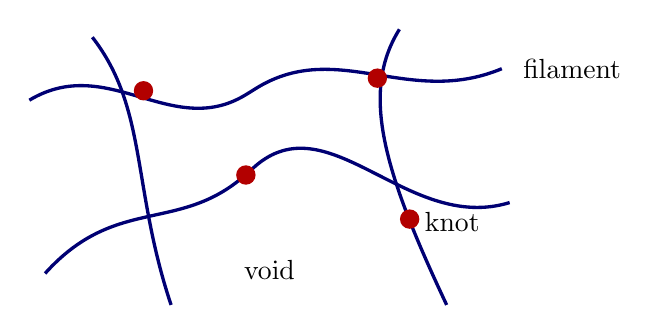
\begin{tikzpicture}[x=1cm,y=1cm]
  \draw[rounded corners=2pt,very thick,blue!45!black]
    (0.2,2.7) .. controls (1.2,3.3) and (2.0,2.2) .. (3.0,2.8)
    .. controls (4.1,3.5) and (5.0,2.6) .. (6.2,3.1);
  \draw[rounded corners=2pt,very thick,blue!45!black]
    (0.4,0.5) .. controls (1.3,1.5) and (2.1,1.0) .. (3.0,1.8)
    .. controls (4.0,2.7) and (5.0,1.0) .. (6.3,1.4);
  \draw[rounded corners=2pt,very thick,blue!45!black]
    (1.0,3.5) .. controls (1.7,2.6) and (1.5,1.6) .. (2.0,0.1);
  \draw[rounded corners=2pt,very thick,blue!45!black]
    (4.9,3.6) .. controls (4.4,2.8) and (4.7,1.8) .. (5.5,0.1);
  \fill[red!70!black] (1.65,2.82) circle (3.5pt);
  \fill[red!70!black] (4.62,2.98) circle (3.5pt);
  \fill[red!70!black] (2.95,1.75) circle (3.5pt);
  \fill[red!70!black] (5.03,1.19) circle (3.5pt);
  \node[align=center] at (3.25,0.55) {void};
  \node[right] at (6.35,3.1) {filament};
  \node[right] at (5.1,1.15) {knot};
\end{tikzpicture}
\caption{焦散网络的一个清晰二维类比：线状聚集包围空洞，并在更亮的结处相交。在三维中，主要折叠是片状结构，其相交形成纤维和节点。}
\label{fig:c09-caustic-network}
\end{figure}

无外力构造并不是宇宙学微扰论的替代品。引力对于密度反差的增长、晕的形成、星系以及非线性结构都至关重要。这个玩具模型分离出一个稳健的几何事实：略微变化的初始流会自然地折叠并聚集。也可以把小的初始密度变化包括进来，而不会改变核心的雅可比论证。

因此，我们只是转移了谜团，而不是消除了它。暴胀被引入，是为了拉伸一个区域，直到它变得极其平坦和均匀。焦散计算假定初始场具有微小的速度变化。那个非均匀的种子从何而来？下一讲将转向暴胀期间场的量子涨落，并追问它们如何成为后来宇宙网的初始条件。

\section{这一论证已确立了什么}

均匀标量场的行为就像在势\(V(\phi)\)中运动的坐标。在固定盒子中，它遵循\(\ddot\phi=-V'(\phi)\)。在膨胀的共动盒子中，物理体积\(a^3\)进入作用量，并产生
\[
\ddot\phi+3H\dot\phi=-V'(\phi).
\]
哈勃摩擦可以把场维持在又高又浅的势上的缓慢终端运动。此时它的动能变得可忽略，它的势能使\(H\)几乎保持恒定，而\(a(t)\)近似指数增长。

膨胀稀释掉不需要的磁单极子，抹平几何，并驱使曲率趋于零。然而暴胀必须结束。场离开平台，发生振荡，并把它的能量转移给再加热产生的高温粒子。若干问题仍然悬而未决：势的形式、暴胀子的身份与初始状态、它的再加热耦合，以及今天观测到的微小真空能。

暴胀的成功引出了最后一个问题。一个被完美抹平的宇宙将不包含任何星系。焦散映射
\[
y=x+v(x)t,
\qquad
\frac{dn}{dy}=\frac{1}{1+v'(x)t}
\]
表明，初始流中的微小变化如何能够生成尖锐的片状结构、纤维状结构和结。它并未解释这些变化的起源。它们的量子起源正是这一论证现在要转向的主题。
